\section{Overview on Development Setup}

A setup for development is explained in table~\ref{tab:requirements}. The most basic components are 
required for hands-on development. Main issue is a python interpreter and common libraries.\footnote{For example
cherrypy, pyserial and optionally a module for SQL-bindings in Python.}

Figure~\ref{setupic} shows the last version of the used development system. The keyboard and monitor on the host machine
is just used to monitor debug output and use the included \textsl{interactive} mode on the \textsc{WSN}.\footnote{So you can 
type in commands meant for nodes on the host machine instead of using the RESTful http-access}

\ref{nodepic} and \ref{hostpic} show the expected results after a clean startup. The controller identifies itself with a
self-chosen name and exchanges basic data for database population.
 

\begin{table}[h] 
\centering 
\begin{tabular}{|l||l|} 
General Component & Specific Component\\ 
\hline 
i86 host machine & 300MHz, 512MB\\ 
host OS & Debian stable(Squeeze) \\ 
Python Interpreter & Python 2.7 with pyserial \\ 
Database & MySQL\footnote{A local sqlite version with reduced functionality has no additional requirements} \\ 
1 Wireless Sensor Node as Controller & Renesas ZMD28-BRD \\
n Wireless Sensor Node as Client & Renesas ZMD28-BRD \\ 
\end{tabular} 
\caption{ Table of Requirements} 
\label{tab:requirements} 
\end{table}


\begin{figure}[H]
   \centering
   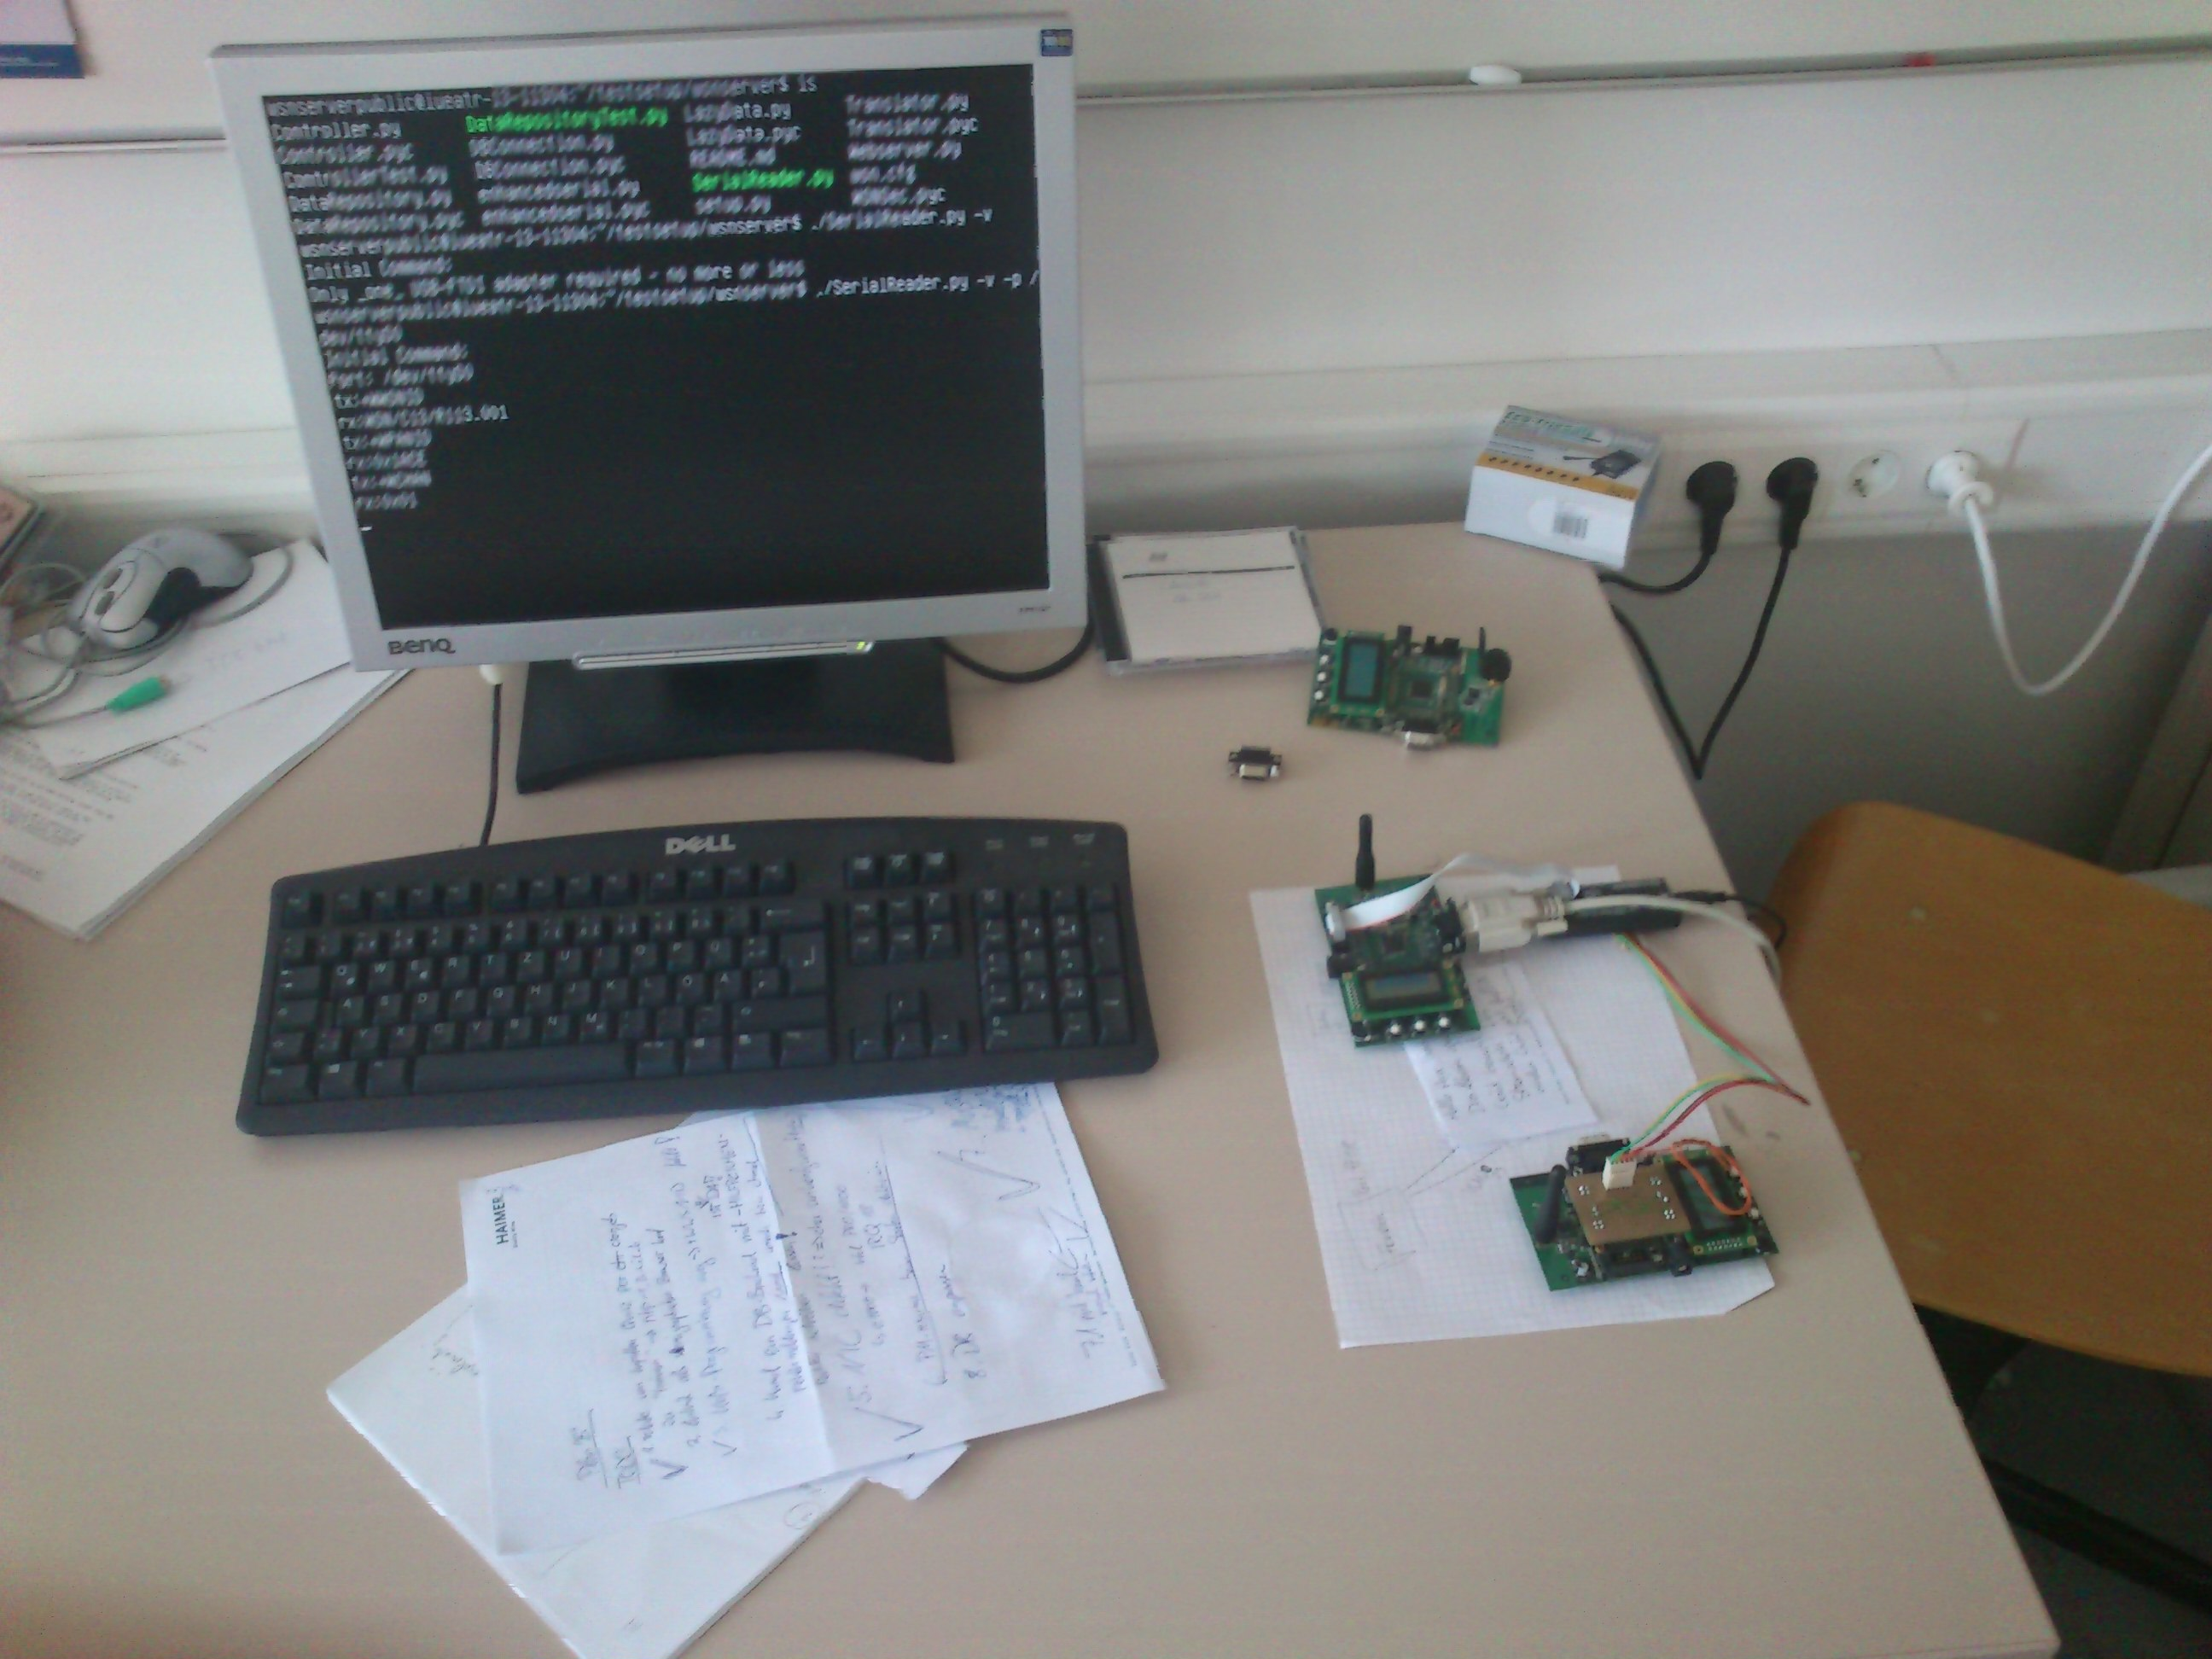
\includegraphics[width=0.8\textwidth]{pic/whole_setup.jpg}%
   \caption{Glimpse on the development setup}
   \label{setupic}%
\end{figure}

-low cost iso available at XXX

\begin{figure}[H]
   \centering
   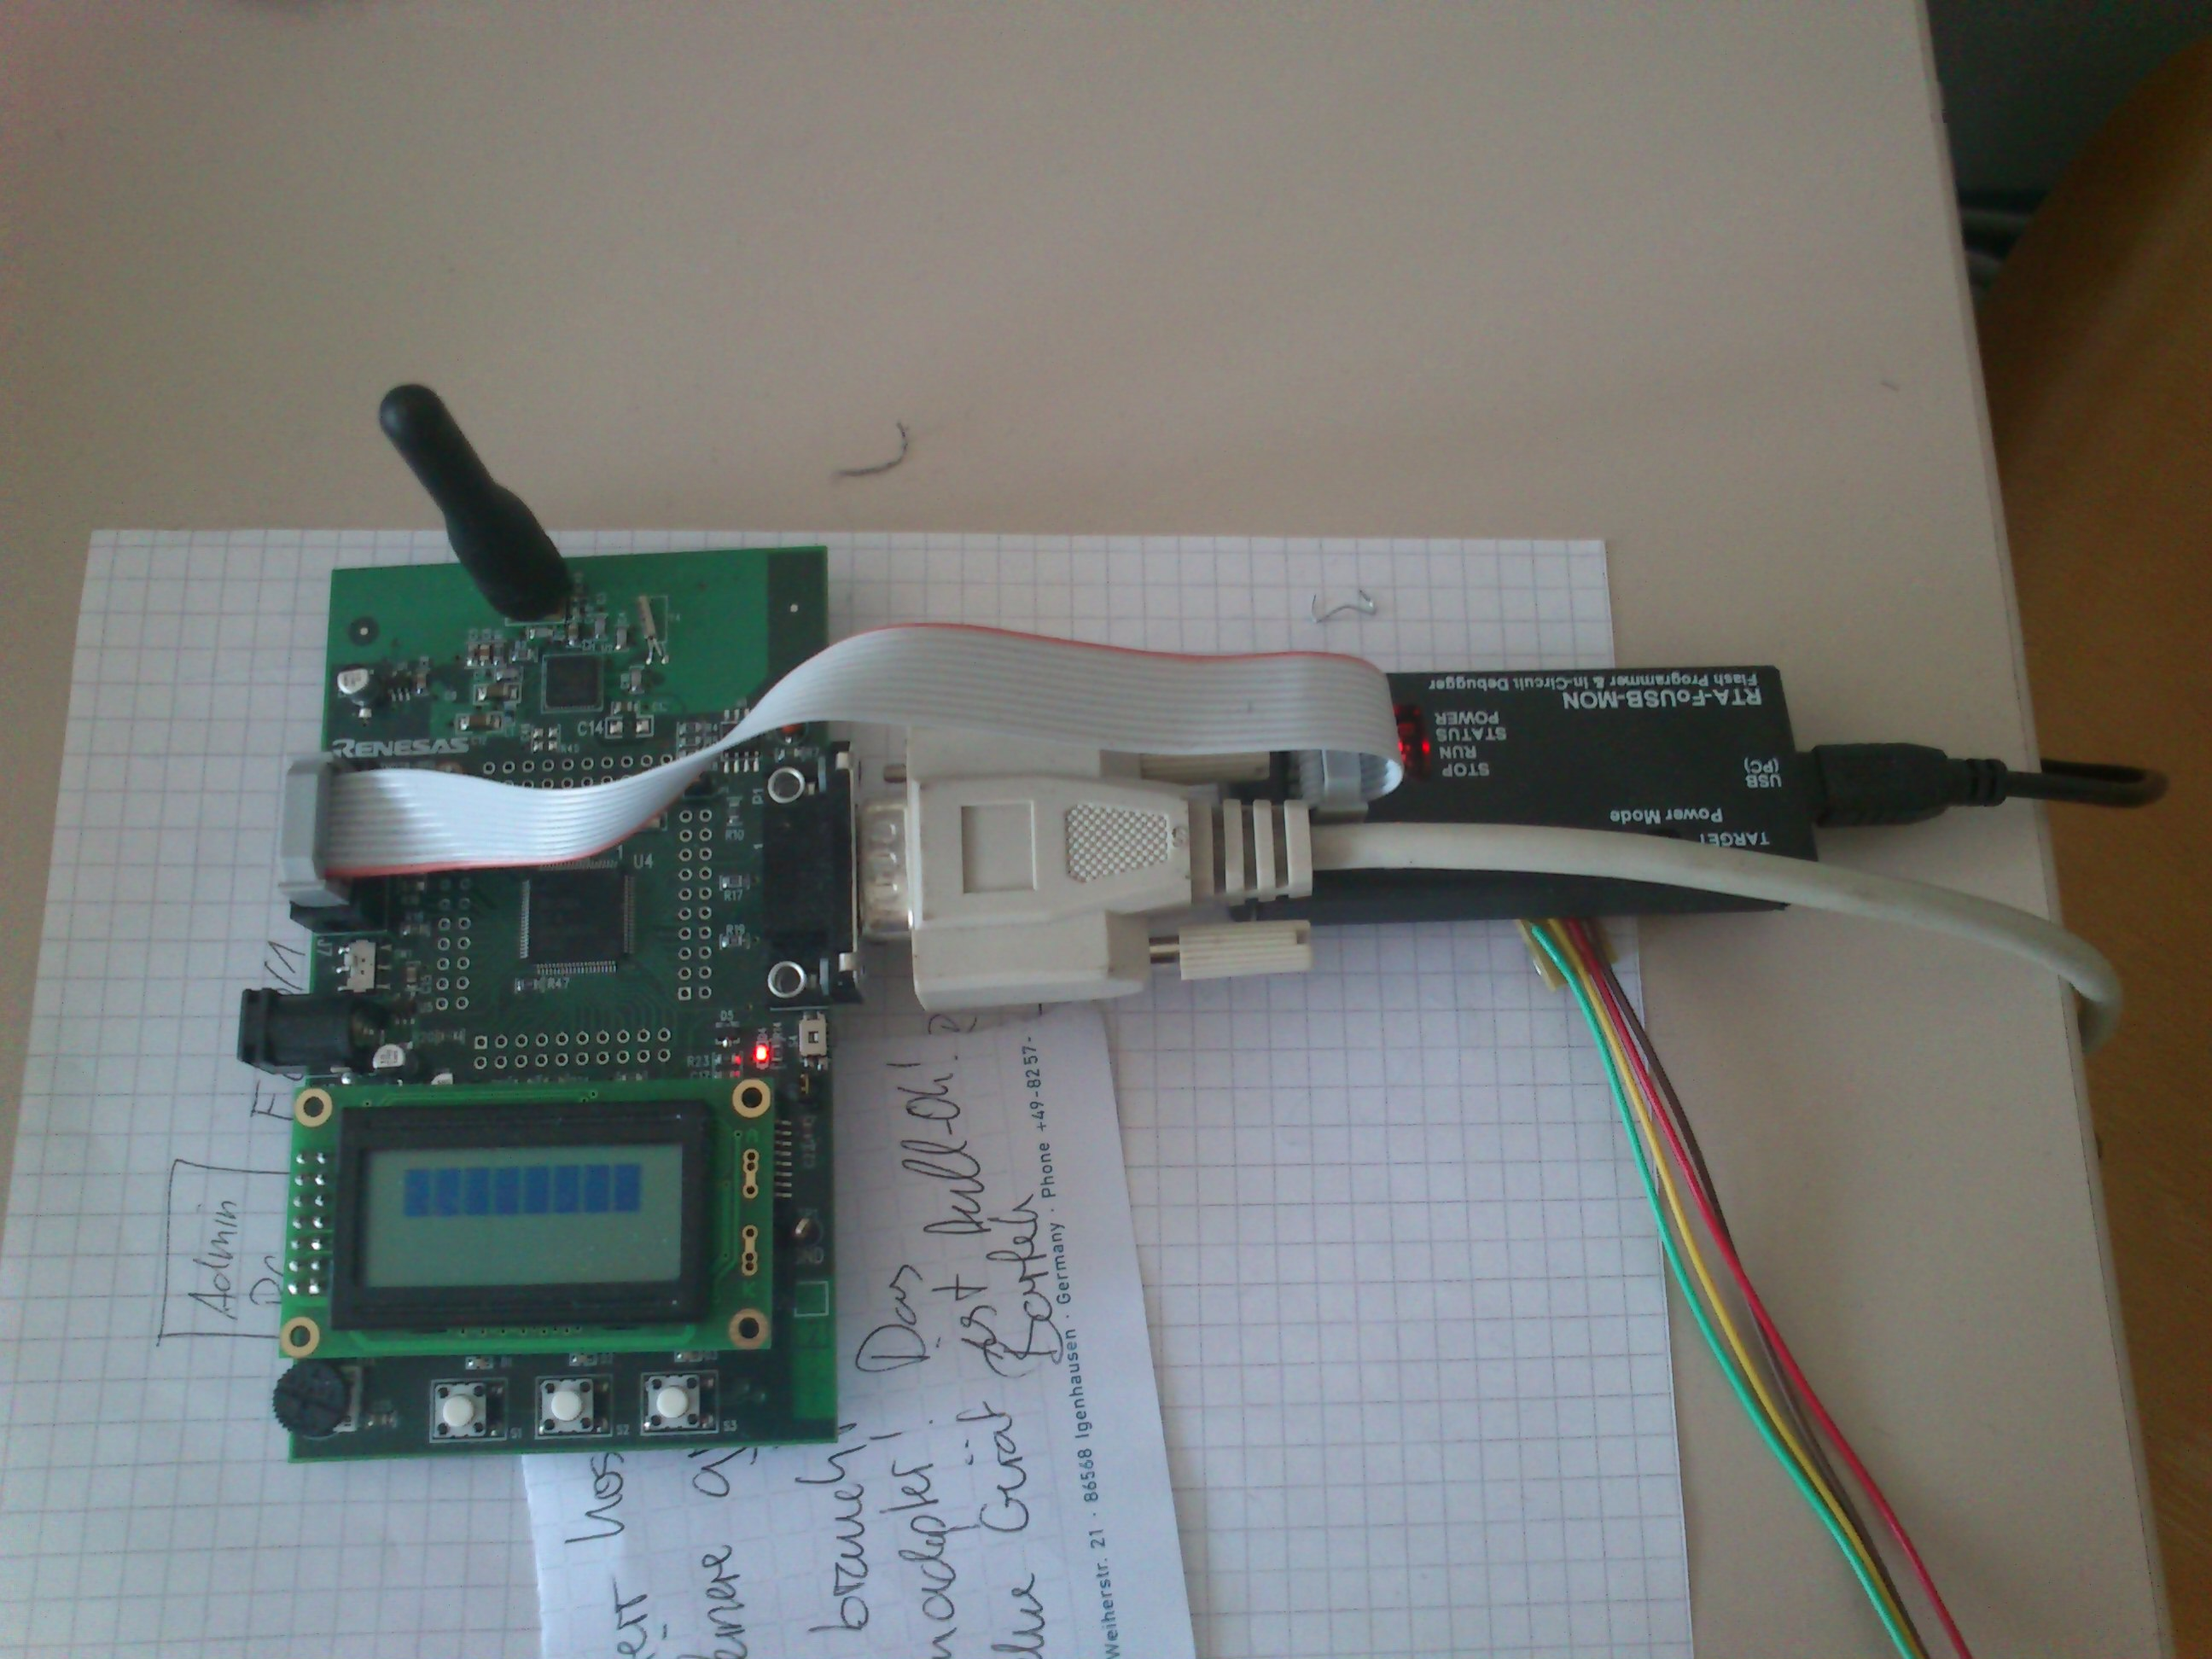
\includegraphics[width=0.8\textwidth]{pic/controller.jpg}%
   \caption{Renesas Node with Custom Programming and Serial Connector}
   \label{nodepic}%
\end{figure}

- less nodes as focused on communication

\begin{figure}[H]
   \centering
   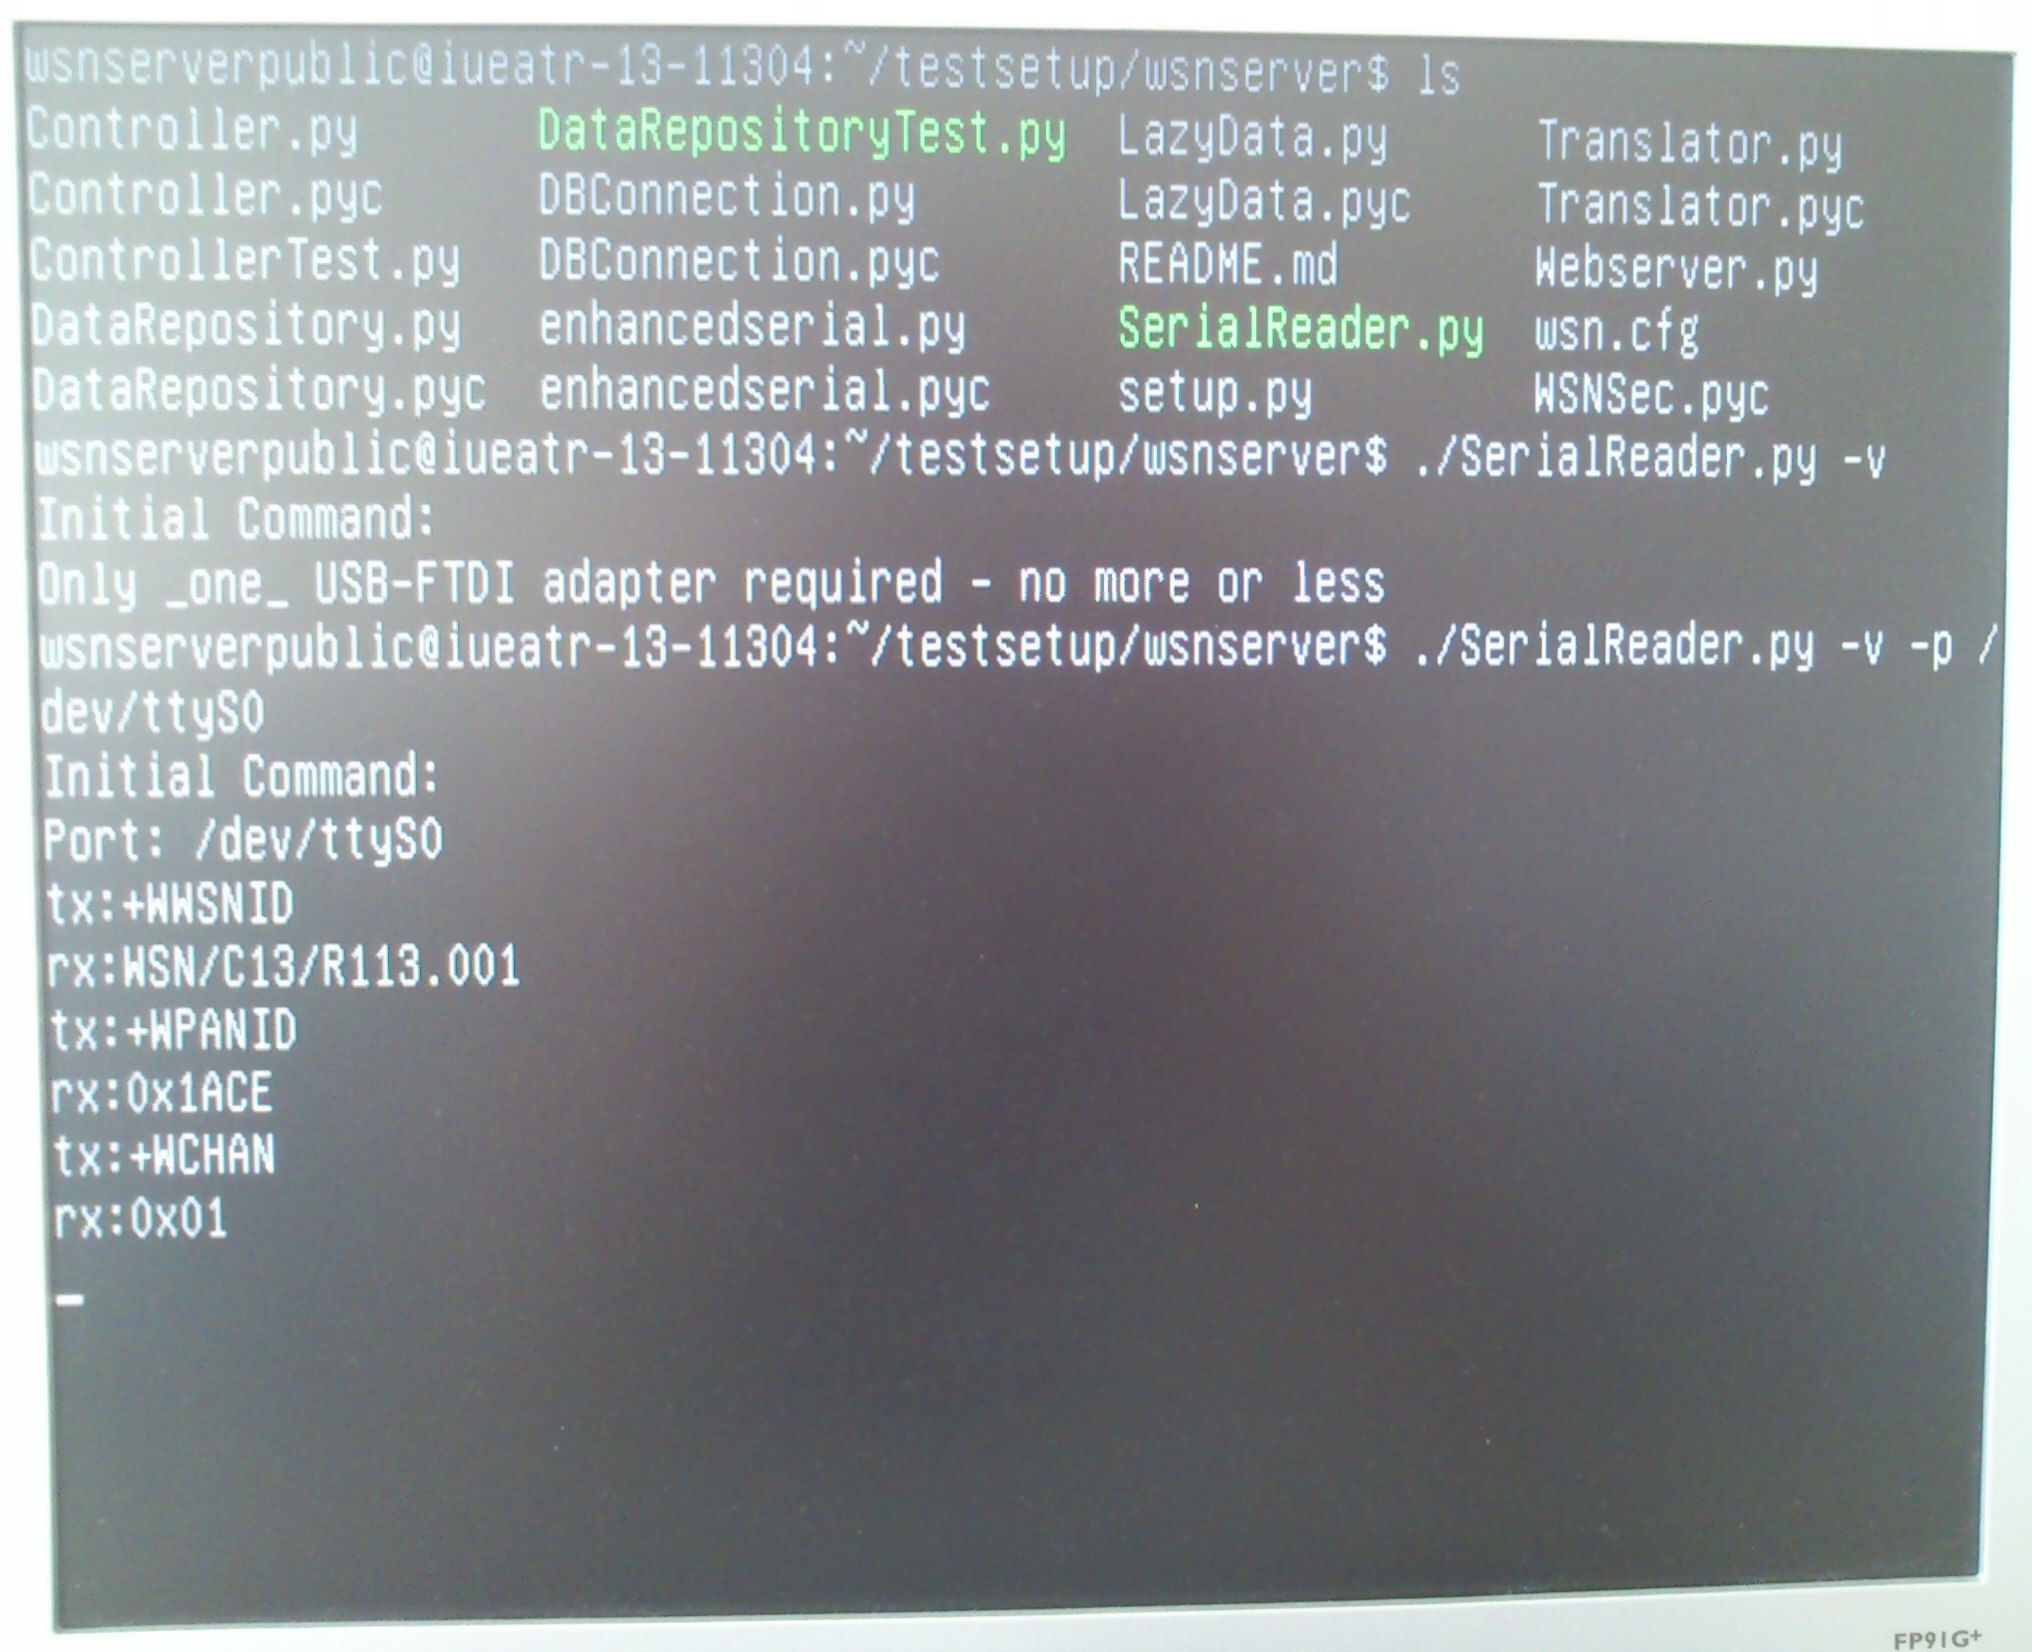
\includegraphics[width=0.8\textwidth]{pic/host_machine.jpg}%
   \caption{Console Output on Host Machine}
   \label{hostpic}%
\end{figure}

- initialisiation description

\newpage
\section{The development method}

For development there have been used different approaches. Most of this project has been developed by the use of agile methods, what means that a feature was implemented and then tested. If it worked properly, it has been committed to a central repository. Critical parts like the "Controller" and the "DataRepository" classes have been developed by using the test-driven-development, where first tests have been written and afterwards the corresponding methods. This last development technique had their advantages and made the expansion of the "DataRepository" class with a second database layer - MySQL - much easier and faster: each test case created for the first database layer - SQLite - had also to work with the newly implemented layer for MySQL.

\section{Class diagrams}
\subsection{The Controller class}
\begin{figure}[H]
   \centering
   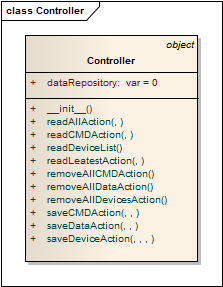
\includegraphics[width=0.5\textwidth]{pic/Controller.png}%
   \caption{The Controller class}
   \label{Controllerpic}%
\end{figure}

The "Controller" class is the central part of this project. It corresponds to the controller part of the Model-View-Controller design pattern.

Like in any other MVC applications the controller receives and handles input and requests of the user and also of any other external modules. 
It validates the input and decides what to do with the data passed to the controller, for example if the controller should save it to the model or retrieve some data from the repository and return it as response.

Applied to this project the "Controller" class receives requests from the webserver to retrieve stored data for a WSN and also to save commands for a WSN in the database, which is used as a queue. The second actor of this class is the "SerialReader" class, which also accesses the controller to save its identification credentials, to pass its read sensor data to the controller for saving and to retrieve new commands from the queue.

The last possible user is the setup script, which accesses the controller for maintenance tasks, like removing all data from the datarepository.



\newpage
\subsection{The ControllerTest class}
\begin{figure}[H]
   \centering
   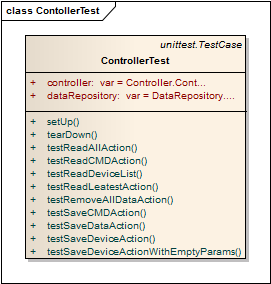
\includegraphics[width=0.5\textwidth]{pic/ControllerTest.png}%
   \caption{ControllerTest class, unittest for the Controller class}
   \label{ControllerTestpic}%
\end{figure}

This unittest was written to test the "Controller" class and their functionality. 

\newpage
\subsection{DataRepository class}
\begin{figure}[H]
   \centering
   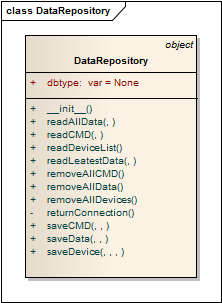
\includegraphics[width=0.5\textwidth]{pic/DataRepository.png}%
   \caption{DataRepository class, which handles the model}
   \label{DataRepositorypic}%
\end{figure}

The "DataRepository" class is the main model class of this project. Their goal is to store and retrieve information and data from the database. Nearly all methods contain SQL instructions, which will be executed by the use of an "DBConnection" object, which contain an actual database connection.

\newpage
\subsection{DataRepositoryTest class}
\begin{figure}[H]
   \centering
   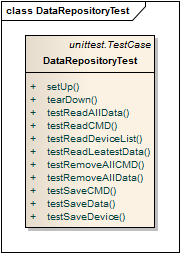
\includegraphics[width=0.5\textwidth]{pic/DataRepositoryTest.png}%
   \caption{DataRepositoryTest class, unittest for the DataRepository class}
   \label{DataRepositoryTestpic}%
\end{figure}

\newpage
\subsection{DBConnection class}
\begin{figure}[H]
   \centering
   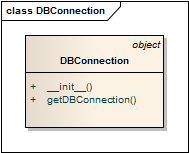
\includegraphics[width=0.5\textwidth]{pic/DBConnection.png}%
   \caption{DBConnection class, a database layer}
   \label{DBConnectionpic}%
\end{figure}

The sole purpose of the "DBConnection" class is to return a open database connection or the caller. 

\newpage
\subsection{EnhancedSerial class}
\begin{figure}[H]
   \centering
   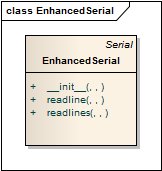
\includegraphics[width=0.5\textwidth]{pic/EnhancedSerial.png}%
   \caption{EnhancedSerial reader class}
   \label{EnhancedSerialpic}%
\end{figure}

\newpage
\subsection{LazyData class}
\begin{figure}[H]
   \centering
   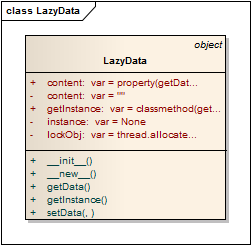
\includegraphics[width=0.5\textwidth]{pic/LazyData.png}%
   \caption{LazyData class}
   \label{LazyDatapic}%
\end{figure}

\newpage
\subsection{Translator class}
\begin{figure}[H]
   \centering
   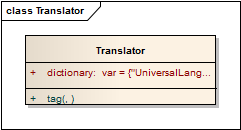
\includegraphics[width=0.5\textwidth]{pic/Translator.png}%
   \caption{Translator class}
   \label{Translatorpic}%
\end{figure}

\subsubsection{MedusaTranslator class}
\begin{figure}[H]
   \centering
   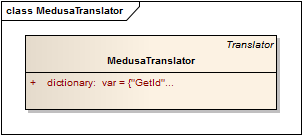
\includegraphics[width=0.5\textwidth]{pic/MedusaTranslator.png}%
   \caption{MedusaTranslator class}
   \label{MedusaTranslatorpic}%
\end{figure}

\subsubsection{RenesasTranslator class}
\begin{figure}[H]
   \centering
   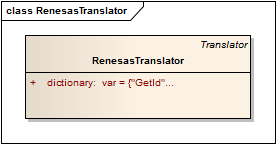
\includegraphics[width=0.5\textwidth]{pic/RenesasTranslator.png}%
   \caption{RenesasTranslator class, dictionary class for Renesas}
   \label{RenesasTranslatorpic}%
\end{figure}

\newpage
\subsection{SerialReader class}
\begin{figure}[H]
   \centering
   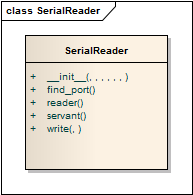
\includegraphics[width=0.5\textwidth]{pic/SerialReader.png}%
   \caption{SerialReader class, main class for reading data from serial port}
   \label{SerialReaderpic}%
\end{figure}

\newpage
\subsection{Webserver class}
\begin{figure}[H]
   \centering
   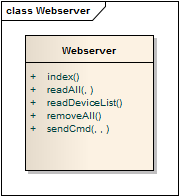
\includegraphics[width=0.5\textwidth]{pic/Webserver.png}%
   \caption{Webserver class, containing the webserver}
   \label{Webserverpic}%
\end{figure}

The "Webserver" class can be seen as the "View" part of the MVC pattern, as it allows and restricts the access and the requests of a user to this specified methods.

The class uses the Cherrypy webserver framework.\footnote{The CherryPy webserver is a open source project hosted on http://www.cherrypy.org/} A standalone webserver written completely in Python. The advantage of this fact is that the dependency of project is reduced to Python instead of the use of a big and resource hungry webserver like Apache2. Also the easy and fast development of methods/pages which comes with the framework.

For demonstrational purpose of the simplicity of CherryPy an extract of the "Webserver" class is presented. As it can bee seen, it is already enough to define a method to receive a functional site. 
\begin{lstlisting}[language=Python]
import Controller
import cherrypy
from cherrypy import expose

class Webserver:
    @expose
    def index(self):
        return "WSN-Server is up and running"
       
\end{lstlisting}

To see if this method works, the user has to call "http://localhost:8080/index" and will receive the status of the webserver.



